\documentclass[1p]{elsarticle_modified}
%\bibliographystyle{elsarticle-num}

%\usepackage[colorlinks]{hyperref}
%\usepackage{abbrmath_seonhwa} %\Abb, \Ascr, \Acal ,\Abf, \Afrak
\usepackage{amsfonts}
\usepackage{amssymb}
\usepackage{amsmath}
\usepackage{amsthm}
\usepackage{scalefnt}
\usepackage{amsbsy}
\usepackage{kotex}
\usepackage{caption}
\usepackage{subfig}
\usepackage{color}
\usepackage{graphicx}
\usepackage{xcolor} %% white, black, red, green, blue, cyan, magenta, yellow
\usepackage{float}
\usepackage{setspace}
\usepackage{hyperref}

\usepackage{tikz}
\usetikzlibrary{arrows}

\usepackage{multirow}
\usepackage{array} % fixed length table
\usepackage{hhline}

%%%%%%%%%%%%%%%%%%%%%
\makeatletter
\renewcommand*\env@matrix[1][\arraystretch]{%
	\edef\arraystretch{#1}%
	\hskip -\arraycolsep
	\let\@ifnextchar\new@ifnextchar
	\array{*\c@MaxMatrixCols c}}
\makeatother %https://tex.stackexchange.com/questions/14071/how-can-i-increase-the-line-spacing-in-a-matrix
%%%%%%%%%%%%%%%

\usepackage[normalem]{ulem}

\newcommand{\msout}[1]{\ifmmode\text{\sout{\ensuremath{#1}}}\else\sout{#1}\fi}
%SOURCE: \msout is \stkout macro in https://tex.stackexchange.com/questions/20609/strikeout-in-math-mode

\newcommand{\cancel}[1]{
	\ifmmode
	{\color{red}\msout{#1}}
	\else
	{\color{red}\sout{#1}}
	\fi
}

\newcommand{\add}[1]{
	{\color{blue}\uwave{#1}}
}

\newcommand{\replace}[2]{
	\ifmmode
	{\color{red}\msout{#1}}{\color{blue}\uwave{#2}}
	\else
	{\color{red}\sout{#1}}{\color{blue}\uwave{#2}}
	\fi
}

\newcommand{\Sol}{\mathcal{S}} %segment
\newcommand{\D}{D} %diagram
\newcommand{\A}{\mathcal{A}} %arc


%%%%%%%%%%%%%%%%%%%%%%%%%%%%%5 test

\def\sl{\operatorname{\textup{SL}}(2,\Cbb)}
\def\psl{\operatorname{\textup{PSL}}(2,\Cbb)}
\def\quan{\mkern 1mu \triangleright \mkern 1mu}

\theoremstyle{definition}
\newtheorem{thm}{Theorem}[section]
\newtheorem{prop}[thm]{Proposition}
\newtheorem{lem}[thm]{Lemma}
\newtheorem{ques}[thm]{Question}
\newtheorem{cor}[thm]{Corollary}
\newtheorem{defn}[thm]{Definition}
\newtheorem{exam}[thm]{Example}
\newtheorem{rmk}[thm]{Remark}
\newtheorem{alg}[thm]{Algorithm}

\newcommand{\I}{\sqrt{-1}}
\begin{document}

%\begin{frontmatter}
%
%\title{Boundary parabolic representations of knots up to 8 crossings}
%
%%% Group authors per affiliation:
%\author{Yunhi Cho} 
%\address{Department of Mathematics, University of Seoul, Seoul, Korea}
%\ead{yhcho@uos.ac.kr}
%
%
%\author{Seonhwa Kim} %\fnref{s_kim}}
%\address{Center for Geometry and Physics, Institute for Basic Science, Pohang, 37673, Korea}
%\ead{ryeona17@ibs.re.kr}
%
%\author{Hyuk Kim}
%\address{Department of Mathematical Sciences, Seoul National University, Seoul 08826, Korea}
%\ead{hyukkim@snu.ac.kr}
%
%\author{Seokbeom Yoon}
%\address{Department of Mathematical Sciences, Seoul National University, Seoul, 08826,  Korea}
%\ead{sbyoon15@snu.ac.kr}
%
%\begin{abstract}
%We find all boundary parabolic representation of knots up to 8 crossings.
%
%\end{abstract}
%\begin{keyword}
%    \MSC[2010] 57M25 
%\end{keyword}
%
%\end{frontmatter}

%\linenumbers
%\tableofcontents
%
\newcommand\colored[1]{\textcolor{white}{\rule[-0.35ex]{0.8em}{1.4ex}}\kern-0.8em\color{red} #1}%
%\newcommand\colored[1]{\textcolor{white}{ #1}\kern-2.17ex	\textcolor{white}{ #1}\kern-1.81ex	\textcolor{white}{ #1}\kern-2.15ex\color{red}#1	}

{\Large $\underline{11a_{366}~(K11a_{366})}$}

\setlength{\tabcolsep}{10pt}
\renewcommand{\arraystretch}{1.6}
\vspace{1cm}\begin{tabular}{m{100pt}>{\centering\arraybackslash}m{274pt}}
\multirow{5}{120pt}{
	\centering
	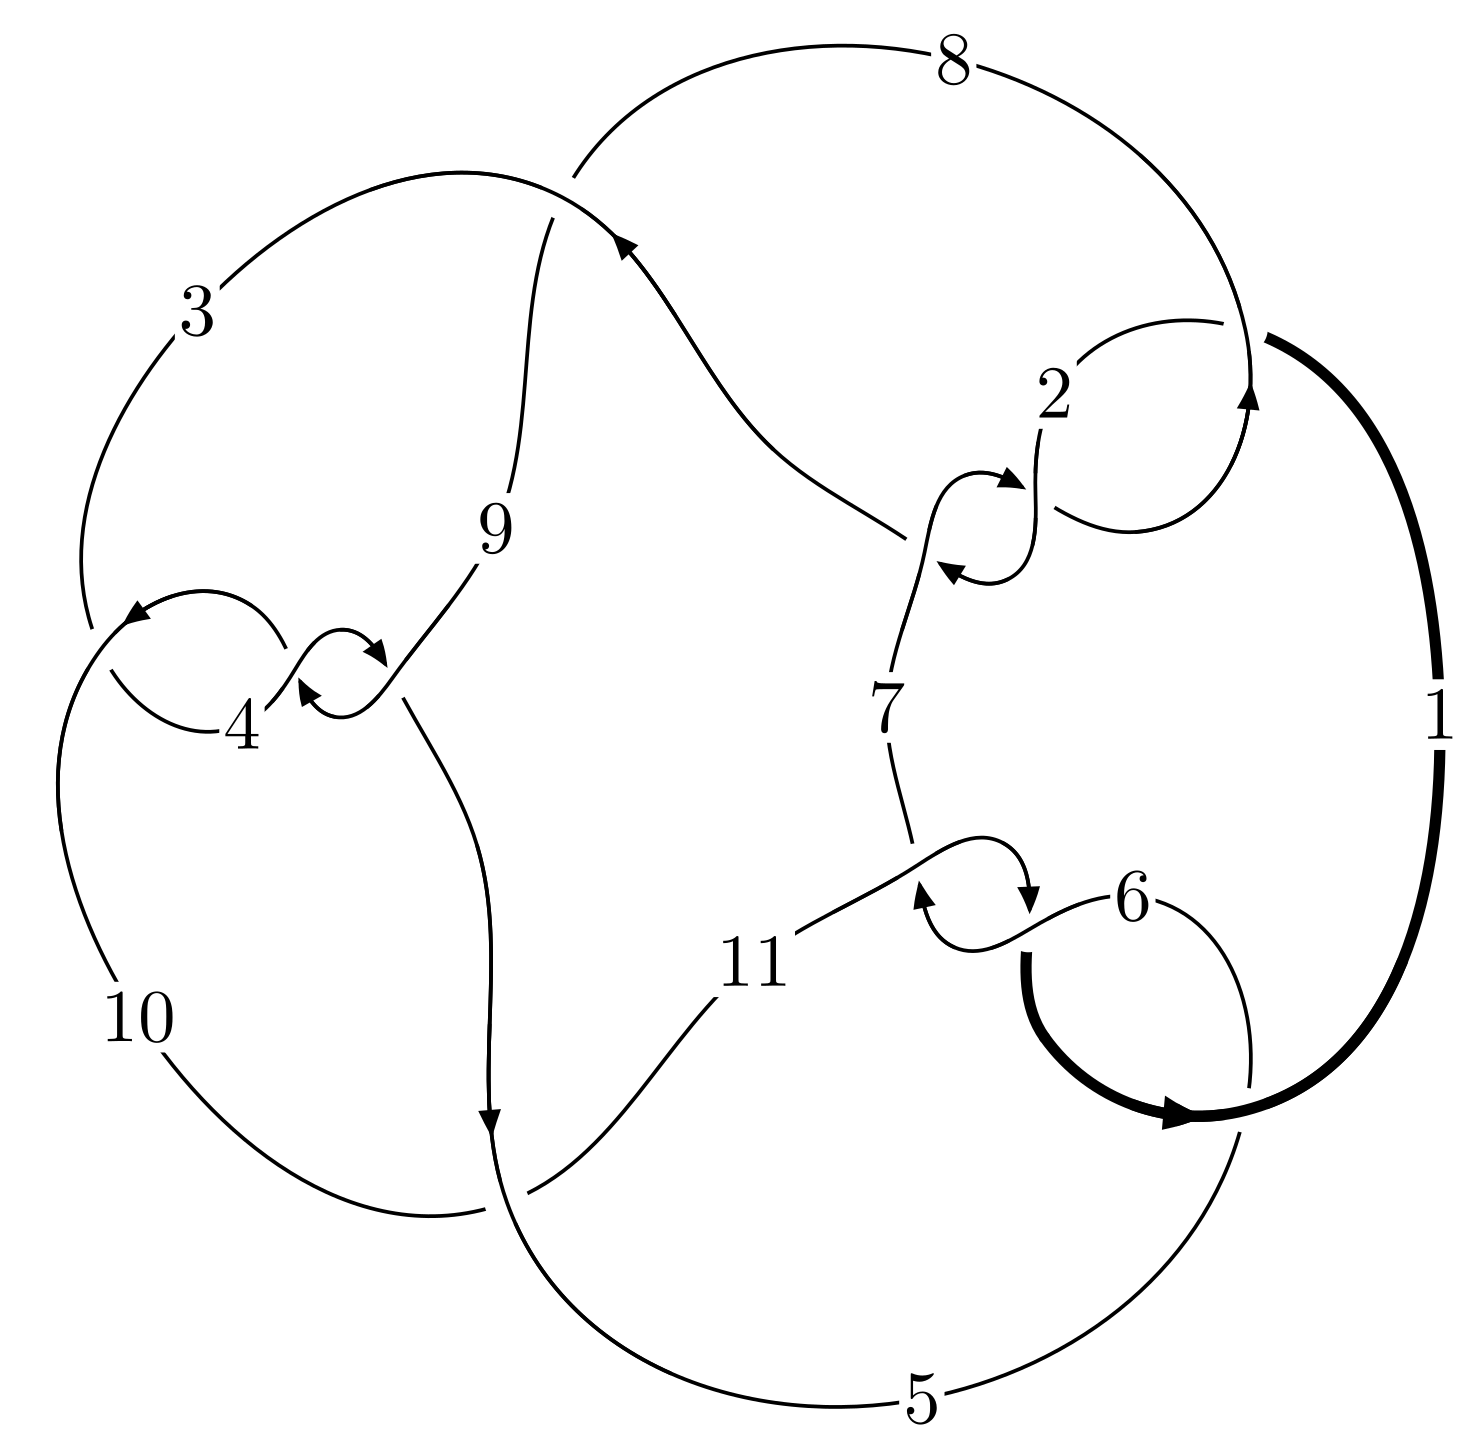
\includegraphics[width=112pt]{../../../GIT/diagram.site/Diagrams/png/615_11a_366.png}\\
\ \ \ A knot diagram\footnotemark}&
\allowdisplaybreaks
\textbf{Linearized knot diagam} \\
\cline{2-2}
 &
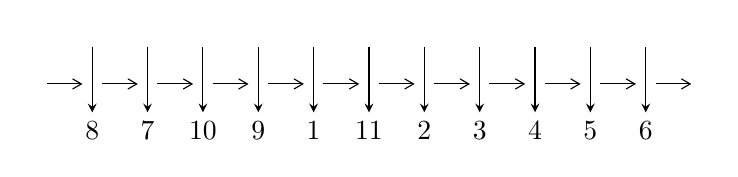
\begin{tikzpicture}[x=20pt, y=17pt]
	% nodes
	\node (C0) at (0, 0) {};
	\node (C1) at (1, 0) {};
	\node (C1U) at (1, +1) {};
	\node (C1D) at (1, -1) {8};

	\node (C2) at (2, 0) {};
	\node (C2U) at (2, +1) {};
	\node (C2D) at (2, -1) {7};

	\node (C3) at (3, 0) {};
	\node (C3U) at (3, +1) {};
	\node (C3D) at (3, -1) {10};

	\node (C4) at (4, 0) {};
	\node (C4U) at (4, +1) {};
	\node (C4D) at (4, -1) {9};

	\node (C5) at (5, 0) {};
	\node (C5U) at (5, +1) {};
	\node (C5D) at (5, -1) {1};

	\node (C6) at (6, 0) {};
	\node (C6U) at (6, +1) {};
	\node (C6D) at (6, -1) {11};

	\node (C7) at (7, 0) {};
	\node (C7U) at (7, +1) {};
	\node (C7D) at (7, -1) {2};

	\node (C8) at (8, 0) {};
	\node (C8U) at (8, +1) {};
	\node (C8D) at (8, -1) {3};

	\node (C9) at (9, 0) {};
	\node (C9U) at (9, +1) {};
	\node (C9D) at (9, -1) {4};

	\node (C10) at (10, 0) {};
	\node (C10U) at (10, +1) {};
	\node (C10D) at (10, -1) {5};

	\node (C11) at (11, 0) {};
	\node (C11U) at (11, +1) {};
	\node (C11D) at (11, -1) {6};
	\node (C12) at (12, 0) {};

	% arrows
	\draw[->,>={angle 60}]
	(C0) edge (C1) (C1) edge (C2) (C2) edge (C3) (C3) edge (C4) (C4) edge (C5) (C5) edge (C6) (C6) edge (C7) (C7) edge (C8) (C8) edge (C9) (C9) edge (C10) (C10) edge (C11) (C11) edge (C12) ;	\draw[->,>=stealth]
	(C1U) edge (C1D) (C2U) edge (C2D) (C3U) edge (C3D) (C4U) edge (C4D) (C5U) edge (C5D) (C6U) edge (C6D) (C7U) edge (C7D) (C8U) edge (C8D) (C9U) edge (C9D) (C10U) edge (C10D) (C11U) edge (C11D) ;
	\end{tikzpicture} \\
\hhline{~~} \\& 
\textbf{Solving Sequence} \\ \cline{2-2} 
 &
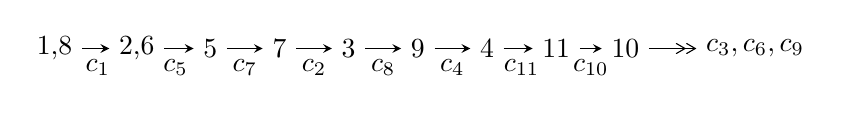
\begin{tikzpicture}[x=25pt, y=7pt]
	% node
	\node (A0) at (-1/8, 0) {1,8};
	\node (A1) at (17/16, 0) {2,6};
	\node (A2) at (17/8, 0) {5};
	\node (A3) at (25/8, 0) {7};
	\node (A4) at (33/8, 0) {3};
	\node (A5) at (41/8, 0) {9};
	\node (A6) at (49/8, 0) {4};
	\node (A7) at (57/8, 0) {11};
	\node (A8) at (65/8, 0) {10};
	\node (C1) at (1/2, -1) {$c_{1}$};
	\node (C2) at (13/8, -1) {$c_{5}$};
	\node (C3) at (21/8, -1) {$c_{7}$};
	\node (C4) at (29/8, -1) {$c_{2}$};
	\node (C5) at (37/8, -1) {$c_{8}$};
	\node (C6) at (45/8, -1) {$c_{4}$};
	\node (C7) at (53/8, -1) {$c_{11}$};
	\node (C8) at (61/8, -1) {$c_{10}$};
	\node (A9) at (10, 0) {$c_{3},c_{6},c_{9}$};

	% edge
	\draw[->,>=stealth]	
	(A0) edge (A1) (A1) edge (A2) (A2) edge (A3) (A3) edge (A4) (A4) edge (A5) (A5) edge (A6) (A6) edge (A7) (A7) edge (A8) ;
	\draw[->>,>={angle 60}]	
	(A8) edge (A9);
\end{tikzpicture} \\ 

\end{tabular} \\

\footnotetext{
The image of knot diagram is generated by the software ``\textbf{Draw programme}" developed by Andrew Bartholomew(\url{http://www.layer8.co.uk/maths/draw/index.htm\#Running-draw}), where we modified some parts for our purpose(\url{https://github.com/CATsTAILs/LinksPainter}).
}\phantom \\ \newline 
\centering \textbf{Ideals for irreducible components\footnotemark of $X_{\text{par}}$} 
 
\begin{align*}
I^u_{1}&=\langle 
b- u,\;- u^5- u^4-3 u^3-2 u^2+a- u,\;u^6+u^5+4 u^4+3 u^3+4 u^2+2 u-1\rangle \\
I^u_{2}&=\langle 
b- u,\;u^9+3 u^7+u^5-4 u^3+a- u+1,\;u^{10}- u^9+5 u^8-5 u^7+9 u^6-9 u^5+6 u^4-6 u^3+u^2+1\rangle \\
I^u_{3}&=\langle 
u^9- u^8+5 u^7-4 u^6+9 u^5-6 u^4+6 u^3-4 u^2+b+u-1,\\
\phantom{I^u_{3}}&\phantom{= \langle  }- u^9+u^8-5 u^7+5 u^6-9 u^5+9 u^4-6 u^3+6 u^2+a- u,\\
\phantom{I^u_{3}}&\phantom{= \langle  }u^{10}- u^9+5 u^8-5 u^7+9 u^6-9 u^5+6 u^4-6 u^3+u^2+1\rangle \\
I^u_{4}&=\langle 
u^9+u^8+3 u^7+2 u^6+3 u^5+2 u^4+2 u^3+2 u^2+b+2 u+1,\\
\phantom{I^u_{4}}&\phantom{= \langle  }- u^9-2 u^8-5 u^7-6 u^6-7 u^5-6 u^4-4 u^3-4 u^2+2 a-3 u-3,\\
\phantom{I^u_{4}}&\phantom{= \langle  }u^{10}+2 u^9+5 u^8+6 u^7+7 u^6+6 u^5+4 u^4+4 u^3+3 u^2+3 u+2\rangle \\
I^u_{5}&=\langle 
b+u,\;a- u+1,\;u^2+1\rangle \\
I^u_{6}&=\langle 
b^2+b u+u^2+1,\;- u^2+a-1,\;u^3+u+1\rangle \\
\\
\end{align*}
\raggedright * 6 irreducible components of $\dim_{\mathbb{C}}=0$, with total 44 representations.\\
\footnotetext{All coefficients of polynomials are rational numbers. But the coefficients are sometimes approximated in decimal forms when there is not enough margin.}
\newpage
\renewcommand{\arraystretch}{1}
\centering \section*{I. $I^u_{1}= \langle b- u,\;- u^5- u^4-3 u^3-2 u^2+a- u,\;u^6+u^5+4 u^4+3 u^3+4 u^2+2 u-1 \rangle$}
\flushleft \textbf{(i) Arc colorings}\\
\begin{tabular}{m{7pt} m{180pt} m{7pt} m{180pt} }
\flushright $a_{1}=$&$\begin{pmatrix}1\\0\end{pmatrix}$ \\
\flushright $a_{8}=$&$\begin{pmatrix}0\\u\end{pmatrix}$ \\
\flushright $a_{2}=$&$\begin{pmatrix}1\\u^2\end{pmatrix}$ \\
\flushright $a_{6}=$&$\begin{pmatrix}u^5+u^4+3 u^3+2 u^2+u\\u\end{pmatrix}$ \\
\flushright $a_{5}=$&$\begin{pmatrix}u^5+u^4+3 u^3+2 u^2+2 u\\u\end{pmatrix}$ \\
\flushright $a_{7}=$&$\begin{pmatrix}u\\u^3+u\end{pmatrix}$ \\
\flushright $a_{3}=$&$\begin{pmatrix}u^2+1\\u^4+2 u^2\end{pmatrix}$ \\
\flushright $a_{9}=$&$\begin{pmatrix}- u^5-2 u^3- u\\- u^4- u^3-2 u^2-2 u+1\end{pmatrix}$ \\
\flushright $a_{4}=$&$\begin{pmatrix}- u^4- u^2+1\\u^5+u^4+2 u^3+2 u^2\end{pmatrix}$ \\
\flushright $a_{11}=$&$\begin{pmatrix}u^4+u^3+3 u^2+2 u\\- u^2\end{pmatrix}$ \\
\flushright $a_{10}=$&$\begin{pmatrix}u^3+2 u\\- u^4-2 u^2\end{pmatrix}$\\ \flushright $a_{10}=$&$\begin{pmatrix}u^3+2 u\\- u^4-2 u^2\end{pmatrix}$\\&\end{tabular}
\flushleft \textbf{(ii) Obstruction class $= -1$}\\~\\
\flushleft \textbf{(iii) Cusp Shapes $= -6 u^4-6 u^3-18 u^2-12 u-16$}\\~\\
\newpage\renewcommand{\arraystretch}{1}
\flushleft \textbf{(iv) u-Polynomials at the component}\newline \\
\begin{tabular}{m{50pt}|m{274pt}}
Crossings & \hspace{64pt}u-Polynomials at each crossing \\
\hline $$\begin{aligned}c_{1},c_{2},c_{3}\\c_{4},c_{5},c_{6}\\c_{7},c_{9},c_{11}\end{aligned}$$&$\begin{aligned}
&u^6- u^5+4 u^4-3 u^3+4 u^2-2 u-1
\end{aligned}$\\
\hline $$\begin{aligned}c_{8},c_{10}\end{aligned}$$&$\begin{aligned}
&u^6+u^5- u^4+3 u^3+4 u^2-12 u-4
\end{aligned}$\\
\hline
\end{tabular}\\~\\
\newpage\renewcommand{\arraystretch}{1}
\flushleft \textbf{(v) Riley Polynomials at the component}\newline \\
\begin{tabular}{m{50pt}|m{274pt}}
Crossings & \hspace{64pt}Riley Polynomials at each crossing \\
\hline $$\begin{aligned}c_{1},c_{2},c_{3}\\c_{4},c_{5},c_{6}\\c_{7},c_{9},c_{11}\end{aligned}$$&$\begin{aligned}
&y^6+7 y^5+18 y^4+17 y^3-4 y^2-12 y+1
\end{aligned}$\\
\hline $$\begin{aligned}c_{8},c_{10}\end{aligned}$$&$\begin{aligned}
&y^6-3 y^5+3 y^4- y^3+96 y^2-176 y+16
\end{aligned}$\\
\hline
\end{tabular}\\~\\
\newpage\flushleft \textbf{(vi) Complex Volumes and Cusp Shapes}
$$\begin{array}{c|c|c}  
\text{Solutions to }I^u_{1}& \I (\text{vol} + \sqrt{-1}CS) & \text{Cusp shape}\\
 \hline 
\begin{aligned}
u &= -0.800464\phantom{ +0.000000I} \\
a &= -0.975734\phantom{ +0.000000I} \\
b &= -0.800464\phantom{ +0.000000I}\end{aligned}
 & -5.50851\phantom{ +0.000000I} & -17.3140\phantom{ +0.000000I} \\ \hline\begin{aligned}
u &= -0.37587 + 1.37813 I \\
a &= -1.38712 - 1.74048 I \\
b &= -0.37587 + 1.37813 I\end{aligned}
 & \phantom{-}7.7894 + 12.7681 I & -4.48012 - 7.54465 I \\ \hline\begin{aligned}
u &= -0.37587 - 1.37813 I \\
a &= -1.38712 + 1.74048 I \\
b &= -0.37587 - 1.37813 I\end{aligned}
 & \phantom{-}7.7894 - 12.7681 I & -4.48012 + 7.54465 I \\ \hline\begin{aligned}
u &= \phantom{-}0.13297 + 1.45639 I \\
a &= \phantom{-}0.61041 - 2.42559 I \\
b &= \phantom{-}0.13297 + 1.45639 I\end{aligned}
 & \phantom{-}14.9383 - 4.7754 I & -0.31743 + 3.39879 I \\ \hline\begin{aligned}
u &= \phantom{-}0.13297 - 1.45639 I \\
a &= \phantom{-}0.61041 + 2.42559 I \\
b &= \phantom{-}0.13297 - 1.45639 I\end{aligned}
 & \phantom{-}14.9383 + 4.7754 I & -0.31743 - 3.39879 I \\ \hline\begin{aligned}
u &= \phantom{-}0.286259\phantom{ +0.000000I} \\
a &= \phantom{-}0.529157\phantom{ +0.000000I} \\
b &= \phantom{-}0.286259\phantom{ +0.000000I}\end{aligned}
 & -0.468566\phantom{ +0.000000I} & -21.0910\phantom{ +0.000000I}\\
 \hline 
 \end{array}$$\newpage\newpage\renewcommand{\arraystretch}{1}
\centering \section*{II. $I^u_{2}= \langle b- u,\;u^9+3 u^7+u^5-4 u^3+a- u+1,\;u^{10}- u^9+\cdots+u^2+1 \rangle$}
\flushleft \textbf{(i) Arc colorings}\\
\begin{tabular}{m{7pt} m{180pt} m{7pt} m{180pt} }
\flushright $a_{1}=$&$\begin{pmatrix}1\\0\end{pmatrix}$ \\
\flushright $a_{8}=$&$\begin{pmatrix}0\\u\end{pmatrix}$ \\
\flushright $a_{2}=$&$\begin{pmatrix}1\\u^2\end{pmatrix}$ \\
\flushright $a_{6}=$&$\begin{pmatrix}- u^9-3 u^7- u^5+4 u^3+u-1\\u\end{pmatrix}$ \\
\flushright $a_{5}=$&$\begin{pmatrix}- u^9-3 u^7- u^5+4 u^3+2 u-1\\u\end{pmatrix}$ \\
\flushright $a_{7}=$&$\begin{pmatrix}u\\u^3+u\end{pmatrix}$ \\
\flushright $a_{3}=$&$\begin{pmatrix}u^2+1\\u^4+2 u^2\end{pmatrix}$ \\
\flushright $a_{9}=$&$\begin{pmatrix}- u^5-2 u^3- u\\- u^7-3 u^5-2 u^3+u\end{pmatrix}$ \\
\flushright $a_{4}=$&$\begin{pmatrix}-2 u^9-8 u^7-10 u^5+u^4- u^3+3 u^2+4 u+1\\- u^9-5 u^7+u^6-9 u^5+4 u^4-5 u^3+5 u^2+2 u+1\end{pmatrix}$ \\
\flushright $a_{11}=$&$\begin{pmatrix}u^9-2 u^8+5 u^7-8 u^6+9 u^5-10 u^4+6 u^3-2 u^2+u\\- u^2\end{pmatrix}$ \\
\flushright $a_{10}=$&$\begin{pmatrix}u^9-2 u^8+5 u^7-8 u^6+9 u^5-11 u^4+6 u^3-5 u^2+u\\- u^4-2 u^2\end{pmatrix}$\\ \flushright $a_{10}=$&$\begin{pmatrix}u^9-2 u^8+5 u^7-8 u^6+9 u^5-11 u^4+6 u^3-5 u^2+u\\- u^4-2 u^2\end{pmatrix}$\\&\end{tabular}
\flushleft \textbf{(ii) Obstruction class $= -1$}\\~\\
\flushleft \textbf{(iii) Cusp Shapes $= 4 u^8+16 u^6-4 u^5+20 u^4-12 u^3+4 u^2-12 u-10$}\\~\\
\newpage\renewcommand{\arraystretch}{1}
\flushleft \textbf{(iv) u-Polynomials at the component}\newline \\
\begin{tabular}{m{50pt}|m{274pt}}
Crossings & \hspace{64pt}u-Polynomials at each crossing \\
\hline $$\begin{aligned}c_{1},c_{2},c_{5}\\c_{6},c_{7},c_{11}\end{aligned}$$&$\begin{aligned}
&u^{10}+u^9+5 u^8+5 u^7+9 u^6+9 u^5+6 u^4+6 u^3+u^2+1
\end{aligned}$\\
\hline $$\begin{aligned}c_{3},c_{4},c_{9}\end{aligned}$$&$\begin{aligned}
&u^{10}-2 u^9+5 u^8-6 u^7+7 u^6-6 u^5+4 u^4-4 u^3+3 u^2-3 u+2
\end{aligned}$\\
\hline $$\begin{aligned}c_{8},c_{10}\end{aligned}$$&$\begin{aligned}
&u^{10}+2 u^9- u^8-5 u^7-3 u^6+4 u^5+12 u^4+13 u^3+5 u^2+u+2
\end{aligned}$\\
\hline
\end{tabular}\\~\\
\newpage\renewcommand{\arraystretch}{1}
\flushleft \textbf{(v) Riley Polynomials at the component}\newline \\
\begin{tabular}{m{50pt}|m{274pt}}
Crossings & \hspace{64pt}Riley Polynomials at each crossing \\
\hline $$\begin{aligned}c_{1},c_{2},c_{5}\\c_{6},c_{7},c_{11}\end{aligned}$$&$\begin{aligned}
&y^{10}+9 y^9+33 y^8+59 y^7+41 y^6-21 y^5-44 y^4-6 y^3+13 y^2+2 y+1
\end{aligned}$\\
\hline $$\begin{aligned}c_{3},c_{4},c_{9}\end{aligned}$$&$\begin{aligned}
&y^{10}+6 y^9+15 y^8+18 y^7+7 y^6-6 y^5-6 y^4+y^2+3 y+4
\end{aligned}$\\
\hline $$\begin{aligned}c_{8},c_{10}\end{aligned}$$&$\begin{aligned}
&y^{10}-6 y^9+\cdots+19 y+4
\end{aligned}$\\
\hline
\end{tabular}\\~\\
\newpage\flushleft \textbf{(vi) Complex Volumes and Cusp Shapes}
$$\begin{array}{c|c|c}  
\text{Solutions to }I^u_{2}& \I (\text{vol} + \sqrt{-1}CS) & \text{Cusp shape}\\
 \hline 
\begin{aligned}
u &= \phantom{-}0.800451 + 0.099834 I \\
a &= \phantom{-}0.984240 + 0.025977 I \\
b &= \phantom{-}0.800451 + 0.099834 I\end{aligned}
 & -1.58679 - 4.14585 I & -12.98134 + 3.97600 I \\ \hline\begin{aligned}
u &= \phantom{-}0.800451 - 0.099834 I \\
a &= \phantom{-}0.984240 - 0.025977 I \\
b &= \phantom{-}0.800451 - 0.099834 I\end{aligned}
 & -1.58679 + 4.14585 I & -12.98134 - 3.97600 I \\ \hline\begin{aligned}
u &= -0.280829 + 1.292560 I \\
a &= -1.76028 - 2.20870 I \\
b &= -0.280829 + 1.292560 I\end{aligned}
 & \phantom{-}5.70347 + 3.47839 I & -4.80497 - 2.79515 I \\ \hline\begin{aligned}
u &= -0.280829 - 1.292560 I \\
a &= -1.76028 + 2.20870 I \\
b &= -0.280829 - 1.292560 I\end{aligned}
 & \phantom{-}5.70347 - 3.47839 I & -4.80497 + 2.79515 I \\ \hline\begin{aligned}
u &= -0.057928 + 1.351670 I \\
a &= -0.46648 - 3.19340 I \\
b &= -0.057928 + 1.351670 I\end{aligned}
 & \phantom{-}8.22706 + 2.31006 I & -3.13631 - 3.52133 I \\ \hline\begin{aligned}
u &= -0.057928 - 1.351670 I \\
a &= -0.46648 + 3.19340 I \\
b &= -0.057928 - 1.351670 I\end{aligned}
 & \phantom{-}8.22706 - 2.31006 I & -3.13631 + 3.52133 I \\ \hline\begin{aligned}
u &= \phantom{-}0.347624 + 1.331990 I \\
a &= \phantom{-}1.56700 - 1.85631 I \\
b &= \phantom{-}0.347624 + 1.331990 I\end{aligned}
 & \phantom{-}2.90872 - 8.28632 I & -8.17560 + 6.14881 I \\ \hline\begin{aligned}
u &= \phantom{-}0.347624 - 1.331990 I \\
a &= \phantom{-}1.56700 + 1.85631 I \\
b &= \phantom{-}0.347624 - 1.331990 I\end{aligned}
 & \phantom{-}2.90872 + 8.28632 I & -8.17560 - 6.14881 I \\ \hline\begin{aligned}
u &= -0.309318 + 0.396943 I \\
a &= -0.824473 + 0.630441 I \\
b &= -0.309318 + 0.396943 I\end{aligned}
 & \phantom{-}2.84181 + 1.23169 I & -8.90177 - 5.44908 I \\ \hline\begin{aligned}
u &= -0.309318 - 0.396943 I \\
a &= -0.824473 - 0.630441 I \\
b &= -0.309318 - 0.396943 I\end{aligned}
 & \phantom{-}2.84181 - 1.23169 I & -8.90177 + 5.44908 I\\
 \hline 
 \end{array}$$\newpage\newpage\renewcommand{\arraystretch}{1}
\centering \section*{III. $I^u_{3}= \langle u^9- u^8+\cdots+b-1,\;- u^9+u^8+\cdots+a- u,\;u^{10}- u^9+\cdots+u^2+1 \rangle$}
\flushleft \textbf{(i) Arc colorings}\\
\begin{tabular}{m{7pt} m{180pt} m{7pt} m{180pt} }
\flushright $a_{1}=$&$\begin{pmatrix}1\\0\end{pmatrix}$ \\
\flushright $a_{8}=$&$\begin{pmatrix}0\\u\end{pmatrix}$ \\
\flushright $a_{2}=$&$\begin{pmatrix}1\\u^2\end{pmatrix}$ \\
\flushright $a_{6}=$&$\begin{pmatrix}u^9- u^8+5 u^7-5 u^6+9 u^5-9 u^4+6 u^3-6 u^2+u\\- u^9+u^8-5 u^7+4 u^6-9 u^5+6 u^4-6 u^3+4 u^2- u+1\end{pmatrix}$ \\
\flushright $a_{5}=$&$\begin{pmatrix}- u^6-3 u^4-2 u^2+1\\- u^9+u^8-5 u^7+4 u^6-9 u^5+6 u^4-6 u^3+4 u^2- u+1\end{pmatrix}$ \\
\flushright $a_{7}=$&$\begin{pmatrix}u\\u^3+u\end{pmatrix}$ \\
\flushright $a_{3}=$&$\begin{pmatrix}u^2+1\\u^4+2 u^2\end{pmatrix}$ \\
\flushright $a_{9}=$&$\begin{pmatrix}- u^5-2 u^3- u\\- u^7-3 u^5-2 u^3+u\end{pmatrix}$ \\
\flushright $a_{4}=$&$\begin{pmatrix}- u^4- u^2+1\\- u^9+2 u^8-5 u^7+7 u^6-9 u^5+8 u^4-6 u^3+3 u^2- u+1\end{pmatrix}$ \\
\flushright $a_{11}=$&$\begin{pmatrix}- u^9-4 u^7-5 u^5+3 u\\- u^7-3 u^5-2 u^3+u^2+u+2\end{pmatrix}$ \\
\flushright $a_{10}=$&$\begin{pmatrix}u^3+2 u\\u^9+3 u^7+2 u^5- u^3+1\end{pmatrix}$\\ \flushright $a_{10}=$&$\begin{pmatrix}u^3+2 u\\u^9+3 u^7+2 u^5- u^3+1\end{pmatrix}$\\&\end{tabular}
\flushleft \textbf{(ii) Obstruction class $= -1$}\\~\\
\flushleft \textbf{(iii) Cusp Shapes $= 4 u^8+16 u^6-4 u^5+20 u^4-12 u^3+4 u^2-12 u-10$}\\~\\
\newpage\renewcommand{\arraystretch}{1}
\flushleft \textbf{(iv) u-Polynomials at the component}\newline \\
\begin{tabular}{m{50pt}|m{274pt}}
Crossings & \hspace{64pt}u-Polynomials at each crossing \\
\hline $$\begin{aligned}c_{1},c_{2},c_{3}\\c_{4},c_{7},c_{9}\end{aligned}$$&$\begin{aligned}
&u^{10}+u^9+5 u^8+5 u^7+9 u^6+9 u^5+6 u^4+6 u^3+u^2+1
\end{aligned}$\\
\hline $$\begin{aligned}c_{5},c_{6},c_{11}\end{aligned}$$&$\begin{aligned}
&u^{10}-2 u^9+5 u^8-6 u^7+7 u^6-6 u^5+4 u^4-4 u^3+3 u^2-3 u+2
\end{aligned}$\\
\hline $$\begin{aligned}c_{8},c_{10}\end{aligned}$$&$\begin{aligned}
&u^{10}+2 u^9- u^8-5 u^7-3 u^6+4 u^5+12 u^4+13 u^3+5 u^2+u+2
\end{aligned}$\\
\hline
\end{tabular}\\~\\
\newpage\renewcommand{\arraystretch}{1}
\flushleft \textbf{(v) Riley Polynomials at the component}\newline \\
\begin{tabular}{m{50pt}|m{274pt}}
Crossings & \hspace{64pt}Riley Polynomials at each crossing \\
\hline $$\begin{aligned}c_{1},c_{2},c_{3}\\c_{4},c_{7},c_{9}\end{aligned}$$&$\begin{aligned}
&y^{10}+9 y^9+33 y^8+59 y^7+41 y^6-21 y^5-44 y^4-6 y^3+13 y^2+2 y+1
\end{aligned}$\\
\hline $$\begin{aligned}c_{5},c_{6},c_{11}\end{aligned}$$&$\begin{aligned}
&y^{10}+6 y^9+15 y^8+18 y^7+7 y^6-6 y^5-6 y^4+y^2+3 y+4
\end{aligned}$\\
\hline $$\begin{aligned}c_{8},c_{10}\end{aligned}$$&$\begin{aligned}
&y^{10}-6 y^9+\cdots+19 y+4
\end{aligned}$\\
\hline
\end{tabular}\\~\\
\newpage\flushleft \textbf{(vi) Complex Volumes and Cusp Shapes}
$$\begin{array}{c|c|c}  
\text{Solutions to }I^u_{3}& \I (\text{vol} + \sqrt{-1}CS) & \text{Cusp shape}\\
 \hline 
\begin{aligned}
u &= \phantom{-}0.800451 + 0.099834 I \\
a &= -1.230160 + 0.153429 I \\
b &= -0.350885 - 1.264620 I\end{aligned}
 & -1.58679 - 4.14585 I & -12.98134 + 3.97600 I \\ \hline\begin{aligned}
u &= \phantom{-}0.800451 - 0.099834 I \\
a &= -1.230160 - 0.153429 I \\
b &= -0.350885 + 1.264620 I\end{aligned}
 & -1.58679 + 4.14585 I & -12.98134 - 3.97600 I \\ \hline\begin{aligned}
u &= -0.280829 + 1.292560 I \\
a &= \phantom{-}0.160513 + 0.738786 I \\
b &= -0.480814 - 1.084510 I\end{aligned}
 & \phantom{-}5.70347 + 3.47839 I & -4.80497 - 2.79515 I \\ \hline\begin{aligned}
u &= -0.280829 - 1.292560 I \\
a &= \phantom{-}0.160513 - 0.738786 I \\
b &= -0.480814 + 1.084510 I\end{aligned}
 & \phantom{-}5.70347 - 3.47839 I & -4.80497 + 2.79515 I \\ \hline\begin{aligned}
u &= -0.057928 + 1.351670 I \\
a &= \phantom{-}0.031648 + 0.738467 I \\
b &= \phantom{-}0.642886 - 0.580182 I\end{aligned}
 & \phantom{-}8.22706 + 2.31006 I & -3.13631 - 3.52133 I \\ \hline\begin{aligned}
u &= -0.057928 - 1.351670 I \\
a &= \phantom{-}0.031648 - 0.738467 I \\
b &= \phantom{-}0.642886 + 0.580182 I\end{aligned}
 & \phantom{-}8.22706 - 2.31006 I & -3.13631 + 3.52133 I \\ \hline\begin{aligned}
u &= \phantom{-}0.347624 + 1.331990 I \\
a &= -0.183438 + 0.702881 I \\
b &= -0.871979 - 0.168588 I\end{aligned}
 & \phantom{-}2.90872 - 8.28632 I & -8.17560 + 6.14881 I \\ \hline\begin{aligned}
u &= \phantom{-}0.347624 - 1.331990 I \\
a &= -0.183438 - 0.702881 I \\
b &= -0.871979 + 0.168588 I\end{aligned}
 & \phantom{-}2.90872 + 8.28632 I & -8.17560 - 6.14881 I \\ \hline\begin{aligned}
u &= -0.309318 + 0.396943 I \\
a &= \phantom{-}1.22144 + 1.56745 I \\
b &= \phantom{-}0.060791 - 1.179490 I\end{aligned}
 & \phantom{-}2.84181 + 1.23169 I & -8.90177 - 5.44908 I \\ \hline\begin{aligned}
u &= -0.309318 - 0.396943 I \\
a &= \phantom{-}1.22144 - 1.56745 I \\
b &= \phantom{-}0.060791 + 1.179490 I\end{aligned}
 & \phantom{-}2.84181 - 1.23169 I & -8.90177 + 5.44908 I\\
 \hline 
 \end{array}$$\newpage\newpage\renewcommand{\arraystretch}{1}
\centering \section*{IV. $I^u_{4}= \langle u^9+u^8+\cdots+b+1,\;- u^9-2 u^8+\cdots+2 a-3,\;u^{10}+2 u^9+\cdots+3 u+2 \rangle$}
\flushleft \textbf{(i) Arc colorings}\\
\begin{tabular}{m{7pt} m{180pt} m{7pt} m{180pt} }
\flushright $a_{1}=$&$\begin{pmatrix}1\\0\end{pmatrix}$ \\
\flushright $a_{8}=$&$\begin{pmatrix}0\\u\end{pmatrix}$ \\
\flushright $a_{2}=$&$\begin{pmatrix}1\\u^2\end{pmatrix}$ \\
\flushright $a_{6}=$&$\begin{pmatrix}\frac{1}{2} u^9+u^8+\cdots+\frac{3}{2} u+\frac{3}{2}\\- u^9- u^8-3 u^7-2 u^6-3 u^5-2 u^4-2 u^3-2 u^2-2 u-1\end{pmatrix}$ \\
\flushright $a_{5}=$&$\begin{pmatrix}-\frac{1}{2} u^9-\frac{1}{2} u^7+\cdots-\frac{1}{2} u+\frac{1}{2}\\- u^9- u^8-3 u^7-2 u^6-3 u^5-2 u^4-2 u^3-2 u^2-2 u-1\end{pmatrix}$ \\
\flushright $a_{7}=$&$\begin{pmatrix}u\\u^3+u\end{pmatrix}$ \\
\flushright $a_{3}=$&$\begin{pmatrix}u^2+1\\u^4+2 u^2\end{pmatrix}$ \\
\flushright $a_{9}=$&$\begin{pmatrix}- u^5-2 u^3- u\\- u^7-3 u^5-2 u^3+u\end{pmatrix}$ \\
\flushright $a_{4}=$&$\begin{pmatrix}\frac{1}{2} u^9+\frac{5}{2} u^7+\cdots-\frac{1}{2} u+\frac{5}{2}\\u^9+3 u^7+3 u^5+2 u^4+u^3+4 u^2+1\end{pmatrix}$ \\
\flushright $a_{11}=$&$\begin{pmatrix}\frac{1}{2} u^9+\frac{3}{2} u^7+\cdots-\frac{1}{2} u+\frac{1}{2}\\u^9+2 u^8+4 u^7+4 u^6+4 u^5+2 u^4+2 u^3+2 u^2+2 u+3\end{pmatrix}$ \\
\flushright $a_{10}=$&$\begin{pmatrix}\frac{1}{2} u^9+\frac{1}{2} u^7+\cdots-\frac{1}{2} u-\frac{1}{2}\\u^9+2 u^8+3 u^7+4 u^6+2 u^5+3 u^4+u^3+2 u^2+2 u+1\end{pmatrix}$\\ \flushright $a_{10}=$&$\begin{pmatrix}\frac{1}{2} u^9+\frac{1}{2} u^7+\cdots-\frac{1}{2} u-\frac{1}{2}\\u^9+2 u^8+3 u^7+4 u^6+2 u^5+3 u^4+u^3+2 u^2+2 u+1\end{pmatrix}$\\&\end{tabular}
\flushleft \textbf{(ii) Obstruction class $= -1$}\\~\\
\flushleft \textbf{(iii) Cusp Shapes $= -4 u^7-8 u^5-4 u^3+4 u-10$}\\~\\
\newpage\renewcommand{\arraystretch}{1}
\flushleft \textbf{(iv) u-Polynomials at the component}\newline \\
\begin{tabular}{m{50pt}|m{274pt}}
Crossings & \hspace{64pt}u-Polynomials at each crossing \\
\hline $$\begin{aligned}c_{1},c_{2},c_{7}\end{aligned}$$&$\begin{aligned}
&u^{10}-2 u^9+5 u^8-6 u^7+7 u^6-6 u^5+4 u^4-4 u^3+3 u^2-3 u+2
\end{aligned}$\\
\hline $$\begin{aligned}c_{3},c_{4},c_{5}\\c_{6},c_{9},c_{11}\end{aligned}$$&$\begin{aligned}
&u^{10}+u^9+5 u^8+5 u^7+9 u^6+9 u^5+6 u^4+6 u^3+u^2+1
\end{aligned}$\\
\hline $$\begin{aligned}c_{8},c_{10}\end{aligned}$$&$\begin{aligned}
&u^{10}+2 u^9- u^8-5 u^7-3 u^6+4 u^5+12 u^4+13 u^3+5 u^2+u+2
\end{aligned}$\\
\hline
\end{tabular}\\~\\
\newpage\renewcommand{\arraystretch}{1}
\flushleft \textbf{(v) Riley Polynomials at the component}\newline \\
\begin{tabular}{m{50pt}|m{274pt}}
Crossings & \hspace{64pt}Riley Polynomials at each crossing \\
\hline $$\begin{aligned}c_{1},c_{2},c_{7}\end{aligned}$$&$\begin{aligned}
&y^{10}+6 y^9+15 y^8+18 y^7+7 y^6-6 y^5-6 y^4+y^2+3 y+4
\end{aligned}$\\
\hline $$\begin{aligned}c_{3},c_{4},c_{5}\\c_{6},c_{9},c_{11}\end{aligned}$$&$\begin{aligned}
&y^{10}+9 y^9+33 y^8+59 y^7+41 y^6-21 y^5-44 y^4-6 y^3+13 y^2+2 y+1
\end{aligned}$\\
\hline $$\begin{aligned}c_{8},c_{10}\end{aligned}$$&$\begin{aligned}
&y^{10}-6 y^9+\cdots+19 y+4
\end{aligned}$\\
\hline
\end{tabular}\\~\\
\newpage\flushleft \textbf{(vi) Complex Volumes and Cusp Shapes}
$$\begin{array}{c|c|c}  
\text{Solutions to }I^u_{4}& \I (\text{vol} + \sqrt{-1}CS) & \text{Cusp shape}\\
 \hline 
\begin{aligned}
u &= -0.871979 + 0.168588 I \\
a &= \phantom{-}1.105490 + 0.213735 I \\
b &= \phantom{-}0.347624 - 1.331990 I\end{aligned}
 & \phantom{-}2.90872 + 8.28632 I & -8.17560 - 6.14881 I \\ \hline\begin{aligned}
u &= -0.871979 - 0.168588 I \\
a &= \phantom{-}1.105490 - 0.213735 I \\
b &= \phantom{-}0.347624 + 1.331990 I\end{aligned}
 & \phantom{-}2.90872 - 8.28632 I & -8.17560 + 6.14881 I \\ \hline\begin{aligned}
u &= \phantom{-}0.642886 + 0.580182 I \\
a &= -0.857280 + 0.773665 I \\
b &= -0.057928 - 1.351670 I\end{aligned}
 & \phantom{-}8.22706 - 2.31006 I & -3.13631 + 3.52133 I \\ \hline\begin{aligned}
u &= \phantom{-}0.642886 - 0.580182 I \\
a &= -0.857280 - 0.773665 I \\
b &= -0.057928 + 1.351670 I\end{aligned}
 & \phantom{-}8.22706 + 2.31006 I & -3.13631 - 3.52133 I \\ \hline\begin{aligned}
u &= \phantom{-}0.060791 + 1.179490 I \\
a &= -0.043581 + 0.845578 I \\
b &= -0.309318 - 0.396943 I\end{aligned}
 & \phantom{-}2.84181 - 1.23169 I & -8.90177 + 5.44908 I \\ \hline\begin{aligned}
u &= \phantom{-}0.060791 - 1.179490 I \\
a &= -0.043581 - 0.845578 I \\
b &= -0.309318 + 0.396943 I\end{aligned}
 & \phantom{-}2.84181 + 1.23169 I & -8.90177 - 5.44908 I \\ \hline\begin{aligned}
u &= -0.480814 + 1.084510 I \\
a &= \phantom{-}0.341647 + 0.770609 I \\
b &= -0.280829 - 1.292560 I\end{aligned}
 & \phantom{-}5.70347 - 3.47839 I & -4.80497 + 2.79515 I \\ \hline\begin{aligned}
u &= -0.480814 - 1.084510 I \\
a &= \phantom{-}0.341647 - 0.770609 I \\
b &= -0.280829 + 1.292560 I\end{aligned}
 & \phantom{-}5.70347 + 3.47839 I & -4.80497 - 2.79515 I \\ \hline\begin{aligned}
u &= -0.350885 + 1.264620 I \\
a &= \phantom{-}0.203721 + 0.734227 I \\
b &= \phantom{-}0.800451 - 0.099834 I\end{aligned}
 & -1.58679 + 4.14585 I & -12.98134 - 3.97600 I \\ \hline\begin{aligned}
u &= -0.350885 - 1.264620 I \\
a &= \phantom{-}0.203721 - 0.734227 I \\
b &= \phantom{-}0.800451 + 0.099834 I\end{aligned}
 & -1.58679 - 4.14585 I & -12.98134 + 3.97600 I\\
 \hline 
 \end{array}$$\newpage\newpage\renewcommand{\arraystretch}{1}
\centering \section*{V. $I^u_{5}= \langle b+u,\;a- u+1,\;u^2+1 \rangle$}
\flushleft \textbf{(i) Arc colorings}\\
\begin{tabular}{m{7pt} m{180pt} m{7pt} m{180pt} }
\flushright $a_{1}=$&$\begin{pmatrix}1\\0\end{pmatrix}$ \\
\flushright $a_{8}=$&$\begin{pmatrix}0\\u\end{pmatrix}$ \\
\flushright $a_{2}=$&$\begin{pmatrix}1\\-1\end{pmatrix}$ \\
\flushright $a_{6}=$&$\begin{pmatrix}u-1\\- u\end{pmatrix}$ \\
\flushright $a_{5}=$&$\begin{pmatrix}-1\\- u\end{pmatrix}$ \\
\flushright $a_{7}=$&$\begin{pmatrix}u\\0\end{pmatrix}$ \\
\flushright $a_{3}=$&$\begin{pmatrix}0\\-1\end{pmatrix}$ \\
\flushright $a_{9}=$&$\begin{pmatrix}0\\u\end{pmatrix}$ \\
\flushright $a_{4}=$&$\begin{pmatrix}-1\\- u-1\end{pmatrix}$ \\
\flushright $a_{11}=$&$\begin{pmatrix}- u\\1\end{pmatrix}$ \\
\flushright $a_{10}=$&$\begin{pmatrix}- u\\1\end{pmatrix}$\\ \flushright $a_{10}=$&$\begin{pmatrix}- u\\1\end{pmatrix}$\\&\end{tabular}
\flushleft \textbf{(ii) Obstruction class $= 1$}\\~\\
\flushleft \textbf{(iii) Cusp Shapes $= -4$}\\~\\
\newpage\renewcommand{\arraystretch}{1}
\flushleft \textbf{(iv) u-Polynomials at the component}\newline \\
\begin{tabular}{m{50pt}|m{274pt}}
Crossings & \hspace{64pt}u-Polynomials at each crossing \\
\hline $$\begin{aligned}c_{1},c_{2},c_{3}\\c_{4},c_{5},c_{6}\\c_{7},c_{9},c_{11}\end{aligned}$$&$\begin{aligned}
&u^2+1
\end{aligned}$\\
\hline $$\begin{aligned}c_{8},c_{10}\end{aligned}$$&$\begin{aligned}
&u^2
\end{aligned}$\\
\hline
\end{tabular}\\~\\
\newpage\renewcommand{\arraystretch}{1}
\flushleft \textbf{(v) Riley Polynomials at the component}\newline \\
\begin{tabular}{m{50pt}|m{274pt}}
Crossings & \hspace{64pt}Riley Polynomials at each crossing \\
\hline $$\begin{aligned}c_{1},c_{2},c_{3}\\c_{4},c_{5},c_{6}\\c_{7},c_{9},c_{11}\end{aligned}$$&$\begin{aligned}
&(y+1)^2
\end{aligned}$\\
\hline $$\begin{aligned}c_{8},c_{10}\end{aligned}$$&$\begin{aligned}
&y^2
\end{aligned}$\\
\hline
\end{tabular}\\~\\
\newpage\flushleft \textbf{(vi) Complex Volumes and Cusp Shapes}
$$\begin{array}{c|c|c}  
\text{Solutions to }I^u_{5}& \I (\text{vol} + \sqrt{-1}CS) & \text{Cusp shape}\\
 \hline 
\begin{aligned}
u &= \phantom{-0.000000 -}1.000000 I \\
a &= -1.00000 + 1.00000 I \\
b &= \phantom{-0.000000 } -1.000000 I\end{aligned}
 & \phantom{-}4.93480\phantom{ +0.000000I} & -4.00000\phantom{ +0.000000I} \\ \hline\begin{aligned}
u &= \phantom{-0.000000 } -1.000000 I \\
a &= -1.00000 - 1.00000 I \\
b &= \phantom{-0.000000 -}1.000000 I\end{aligned}
 & \phantom{-}4.93480\phantom{ +0.000000I} & -4.00000\phantom{ +0.000000I}\\
 \hline 
 \end{array}$$\newpage\newpage\renewcommand{\arraystretch}{1}
\centering \section*{VI. $I^u_{6}= \langle b^2+b u+u^2+1,\;- u^2+a-1,\;u^3+u+1 \rangle$}
\flushleft \textbf{(i) Arc colorings}\\
\begin{tabular}{m{7pt} m{180pt} m{7pt} m{180pt} }
\flushright $a_{1}=$&$\begin{pmatrix}1\\0\end{pmatrix}$ \\
\flushright $a_{8}=$&$\begin{pmatrix}0\\u\end{pmatrix}$ \\
\flushright $a_{2}=$&$\begin{pmatrix}1\\u^2\end{pmatrix}$ \\
\flushright $a_{6}=$&$\begin{pmatrix}u^2+1\\b\end{pmatrix}$ \\
\flushright $a_{5}=$&$\begin{pmatrix}u^2+b+1\\b\end{pmatrix}$ \\
\flushright $a_{7}=$&$\begin{pmatrix}u\\-1\end{pmatrix}$ \\
\flushright $a_{3}=$&$\begin{pmatrix}u^2+1\\u^2- u\end{pmatrix}$ \\
\flushright $a_{9}=$&$\begin{pmatrix}u^2+1\\u^2\end{pmatrix}$ \\
\flushright $a_{4}=$&$\begin{pmatrix}u^2 b+u^2+2 b\\u^2 b+b- u-1\end{pmatrix}$ \\
\flushright $a_{11}=$&$\begin{pmatrix}- u^2 b- b+1\\b u+u^2+1\end{pmatrix}$ \\
\flushright $a_{10}=$&$\begin{pmatrix}- u^2 b+u^2+2\\b u+u^2+b+1\end{pmatrix}$\\ \flushright $a_{10}=$&$\begin{pmatrix}- u^2 b+u^2+2\\b u+u^2+b+1\end{pmatrix}$\\&\end{tabular}
\flushleft \textbf{(ii) Obstruction class $= -1$}\\~\\
\flushleft \textbf{(iii) Cusp Shapes $= -10$}\\~\\
\newpage\renewcommand{\arraystretch}{1}
\flushleft \textbf{(iv) u-Polynomials at the component}\newline \\
\begin{tabular}{m{50pt}|m{274pt}}
Crossings & \hspace{64pt}u-Polynomials at each crossing \\
\hline $$\begin{aligned}c_{1},c_{2},c_{3}\\c_{4},c_{5},c_{6}\\c_{7},c_{9},c_{11}\end{aligned}$$&$\begin{aligned}
&(u^3+u-1)^2
\end{aligned}$\\
\hline $$\begin{aligned}c_{8},c_{10}\end{aligned}$$&$\begin{aligned}
&(u-1)^6
\end{aligned}$\\
\hline
\end{tabular}\\~\\
\newpage\renewcommand{\arraystretch}{1}
\flushleft \textbf{(v) Riley Polynomials at the component}\newline \\
\begin{tabular}{m{50pt}|m{274pt}}
Crossings & \hspace{64pt}Riley Polynomials at each crossing \\
\hline $$\begin{aligned}c_{1},c_{2},c_{3}\\c_{4},c_{5},c_{6}\\c_{7},c_{9},c_{11}\end{aligned}$$&$\begin{aligned}
&(y^3+2 y^2+y-1)^2
\end{aligned}$\\
\hline $$\begin{aligned}c_{8},c_{10}\end{aligned}$$&$\begin{aligned}
&(y-1)^6
\end{aligned}$\\
\hline
\end{tabular}\\~\\
\newpage\flushleft \textbf{(vi) Complex Volumes and Cusp Shapes}
$$\begin{array}{c|c|c}  
\text{Solutions to }I^u_{6}& \I (\text{vol} + \sqrt{-1}CS) & \text{Cusp shape}\\
 \hline 
\begin{aligned}
u &= \phantom{-}0.341164 + 1.161540 I \\
a &= -0.232786 + 0.792552 I \\
b &= \phantom{-}0.341164 - 1.161540 I\end{aligned}
 & \phantom{-}1.64493\phantom{ +0.000000I} & -10.0000\phantom{ +0.000000I} \\ \hline\begin{aligned}
u &= \phantom{-}0.341164 + 1.161540 I \\
a &= -0.232786 + 0.792552 I \\
b &= -0.682328\phantom{ +0.000000I}\end{aligned}
 & \phantom{-}1.64493\phantom{ +0.000000I} & -10.0000\phantom{ +0.000000I} \\ \hline\begin{aligned}
u &= \phantom{-}0.341164 - 1.161540 I \\
a &= -0.232786 - 0.792552 I \\
b &= \phantom{-}0.341164 + 1.161540 I\end{aligned}
 & \phantom{-}1.64493\phantom{ +0.000000I} & -10.0000\phantom{ +0.000000I} \\ \hline\begin{aligned}
u &= \phantom{-}0.341164 - 1.161540 I \\
a &= -0.232786 - 0.792552 I \\
b &= -0.682328\phantom{ +0.000000I}\end{aligned}
 & \phantom{-}1.64493\phantom{ +0.000000I} & -10.0000\phantom{ +0.000000I} \\ \hline\begin{aligned}
u &= -0.682328\phantom{ +0.000000I} \\
a &= \phantom{-}1.46557\phantom{ +0.000000I} \\
b &= \phantom{-}0.341164 + 1.161540 I\end{aligned}
 & \phantom{-}1.64493\phantom{ +0.000000I} & -10.0000\phantom{ +0.000000I} \\ \hline\begin{aligned}
u &= -0.682328\phantom{ +0.000000I} \\
a &= \phantom{-}1.46557\phantom{ +0.000000I} \\
b &= \phantom{-}0.341164 - 1.161540 I\end{aligned}
 & \phantom{-}1.64493\phantom{ +0.000000I} & -10.0000\phantom{ +0.000000I}\\
 \hline 
 \end{array}$$\newpage
\newpage\renewcommand{\arraystretch}{1}
\centering \section*{ VII. u-Polynomials}
\begin{tabular}{m{50pt}|m{274pt}}
Crossings & \hspace{64pt}u-Polynomials at each crossing \\
\hline $$\begin{aligned}c_{1},c_{2},c_{3}\\c_{4},c_{5},c_{6}\\c_{7},c_{9},c_{11}\end{aligned}$$&$\begin{aligned}
&(u^2+1)(u^3+u-1)^2(u^6- u^5+4 u^4-3 u^3+4 u^2-2 u-1)\\
&\cdot(u^{10}-2 u^9+5 u^8-6 u^7+7 u^6-6 u^5+4 u^4-4 u^3+3 u^2-3 u+2)\\
&\cdot(u^{10}+u^9+5 u^8+5 u^7+9 u^6+9 u^5+6 u^4+6 u^3+u^2+1)^2
\end{aligned}$\\
\hline $$\begin{aligned}c_{8},c_{10}\end{aligned}$$&$\begin{aligned}
&u^2(u-1)^6(u^6+u^5- u^4+3 u^3+4 u^2-12 u-4)\\
&\cdot(u^{10}+2 u^9- u^8-5 u^7-3 u^6+4 u^5+12 u^4+13 u^3+5 u^2+u+2)^3
\end{aligned}$\\
\hline
\end{tabular}\newpage\renewcommand{\arraystretch}{1}
\centering \section*{ VIII. Riley Polynomials}
\begin{tabular}{m{50pt}|m{274pt}}
Crossings & \hspace{64pt}Riley Polynomials at each crossing \\
\hline $$\begin{aligned}c_{1},c_{2},c_{3}\\c_{4},c_{5},c_{6}\\c_{7},c_{9},c_{11}\end{aligned}$$&$\begin{aligned}
&((y+1)^2)(y^3+2 y^2+y-1)^2(y^6+7 y^5+\cdots-12 y+1)\\
&\cdot(y^{10}+6 y^9+15 y^8+18 y^7+7 y^6-6 y^5-6 y^4+y^2+3 y+4)\\
&\cdot(y^{10}+9 y^9+33 y^8+59 y^7+41 y^6-21 y^5-44 y^4-6 y^3+13 y^2+2 y+1)^{2}
\end{aligned}$\\
\hline $$\begin{aligned}c_{8},c_{10}\end{aligned}$$&$\begin{aligned}
&y^2(y-1)^6(y^6-3 y^5+3 y^4- y^3+96 y^2-176 y+16)\\
&\cdot(y^{10}-6 y^9+\cdots+19 y+4)^{3}
\end{aligned}$\\
\hline
\end{tabular}
\vskip 2pc
\end{document}